% This must be in the first 5 lines to tell arXiv to use pdfLaTeX, which is strongly recommended.
\pdfoutput=1
% In particular, the hyperref package requires pdfLaTeX in order to break URLs across lines.

\documentclass[11pt]{article}

% Change "review" to "final" to generate the final (sometimes called camera-ready) version.
% Change to "preprint" to generate a non-anonymous version with page numbers.
\usepackage[preprint]{acl}

% Standard package includes
\usepackage{times}
\usepackage{latexsym}

% For proper rendering and hyphenation of words containing Latin characters (including in bib files)
\usepackage[T1]{fontenc}

% This assumes your files are encoded as UTF8
\usepackage[utf8]{inputenc}

% This is not strictly necessary, and may be commented out,
% but it will improve the layout of the manuscript,
% and will typically save some space.
\usepackage{microtype}

% This is also not strictly necessary, and may be commented out.
% However, it will improve the aesthetics of text in
% the typewriter font.
\usepackage{inconsolata}
\usepackage{graphicx}

\usepackage{listings}
\usepackage{xcolor}

\lstset{
	basicstyle=\ttfamily\small,   % Monospace font with small size
	keywordstyle=\color{blue},    % Keywords in blue
	commentstyle=\color{green!50!black}, % Comments in green
	stringstyle=\color{red},      % Strings in red
	numbers=left,                 % Line numbers on the left
	numberstyle=\tiny\color{gray},% Line number styling
	frame=lines,                  % Add a frame around the code
	breaklines=true,              % Allow line breaks
	captionpos=b,                 % Caption below the listing
	tabsize=4,                    % Set tab size
	showstringspaces=false,       % Don't show spaces in strings
}



\title{Exploring Methods for Efficient Fine-tuning of LLMs for Semantic Evaluation}
\author{
	Nicholas Boddy \and Caleb Raschka \and Morgan Turville-Heitz \\
	\textit{University of Wisconsin-Madison}
}
\date{\today}


\begin{document}
\maketitle

\begin{center}
	\textit{Project Report for CS 769 - Advanced Natural Language Processing}
\end{center}

\section{Introduction}

LoRA is a powerful method for the fine-tuning of LLMs (and large models in general) on lower end hardware. As students, engaging with modern machine learning research can be challenging; many of us are limited in computational resources to at best a single commercial CUDA-compatible GPU. For this reason, efficient fine-tuning is exceptionally enticing. We therefore chose to reimplement LoRA as the first part of our project, with further goals of exploring other fine-tuning methods like QLoRA. We show that LoRA and QLoRA can make large scale LLM work accessible to students and researchers limited to consumer hardware, based off the metric of efficient semantic evaluation. In particular, we have reimplemented the fine-tuning of Llama 2 - 7B and Llama 3.2 - 1B via LoRA, similar to the implementation shown in \cite{hu2021lora}, as well as implementing LoRA for fine-tuning, as shown in \cite{dettmers2023qlora}. This work exhibits the capabilities of LoRA and QLoRA for the fine-tuning of models on at-home hardware, which is a standard limitation for LLMs. In addition to the reduction in memory requirements under LoRA and QLoRA, we also show significant improvements in training time per epoch, with minimal loss in model accuracy following fine-tuning.

With both our LoRA and QLoRA implementation, we have been able to meet baseline performance on the F1-Macro and F1-Micro metrics for the SEMEVAL 2021 task 6\footnote{Task: propaganda.math.unipd.it/semeval2021task6/}. SEMEVAL 2021 task 6, titled “Detection of Persuasive Techniques in Texts and Images,” concerns the semantic identification of forms of propagandistic narratives used in memes. In particular, the task is concerned with which, if any, of 20 forms of narrative technique is utilized in the meme in order to convey an agenda. We have approached subtask 1 in particular, because subtask 2 and subtask 3 will require more computing resources than we have access to, and would require multi-modal implementation of the fine-tuned model.

In order to achieve these goals, we worked with LLM models with sizes appropriate for our at-home resources. We implemented two mid-sized models, Llama 2 - 7B and Llama 3.2 - 1B. These were fine-tuned off of the SEMEVAL 2021 Task 6 datasets\footnote{Data: github.com/di-dimitrov/SEMEVAL-2021-task6-corpus/tree/main/data} for subtask 1, with the end-goal of predicting the form of propagandistic technique in the original meme. Our results for each model are shown in the Results section, which we compare against the literature results, and are also compared against the leaderboard for the task. We find that the implementation of QLoRA further increases the capacity for model sizes that we are able to fine tune.

In addition to comparing accuracies of these models against those on the existing leaderboards, we compare both training times and inference times between the models to judge how effectively efficient the various fine-tuning methods are. We include results for the full fine-tuned (FFT) model in order to contrast performance with LoRA and QLoRA.

\begin{figure*}[h]
	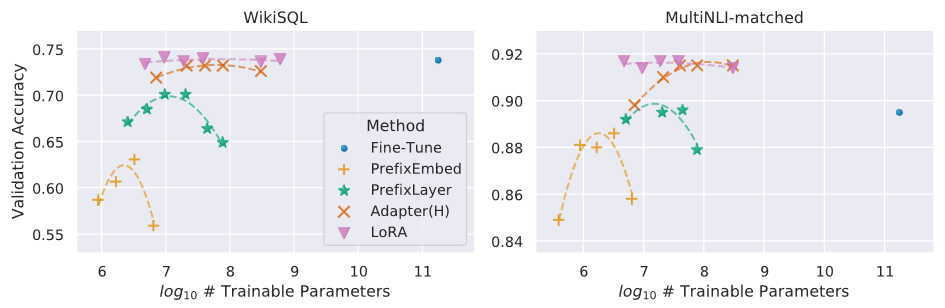
\includegraphics[width=6in]{finetuning_scalability.png}
	\centering
	\caption{LoRA exhibits both better scalability and task performance in comparison to alternative parameter-efficient fine-tuning methods. Additionally, task performance is measured to meet, if not exceed that of full fine-tuning. \cite{hu2021lora}}
	\label{fig:ft_scale}
\end{figure*}

\section{Related Literature}

The efficient adaptation of large language models (LLMs) has become increasingly important as models grow in size and computational requirements. \cite{hu2021lora} introduced LoRA (Low-Rank Adaptation), a foundational method that significantly reduces the memory and computational costs of fine-tuning LLMs. LoRA works by freezing the pretrained model weights and injecting trainable rank decomposition matrices into each layer of the transformer architecture. This approach reduces the number of trainable parameters by several orders of magnitude while maintaining model quality comparable to the FFT performance. The key insight of LoRA is that the changes in weights during model adaptation have a low "intrinsic rank," allowing for effective parameter-efficient fine-tuning.

Building on Hu et al.’s prior work, \cite{he2022unified} provided a unified framework for parameter-efficient tuning methods. Through analysis of adapters, prefix tuning, and LoRA, they showed these methods still lagged behind FFT on challenging tasks like summarization and machine translation. By demonstrating that prefix tuning could be reformulated as a form of adapter, they identified key design dimensions across methods. Their experiments on diverse benchmarks led to the Mix-and-Match (MaM) Adapter, which matched FFT performance while using only 6.7\% of trainable parameters on generation tasks and 0.5\% on classification tasks \cite{he2022unified}.


Further advancements on the low rank adaptation methodology were made by \cite{dettmers2023qlora}, advancing the field further last year with QLoRA, which combines quantization with LoRA to achieve even greater memory efficiency. QLoRA introduces several innovations, including 4-bit NormalFloat quantization (optimized for normally distributed weights), double quantization (which quantizes the quantization constants), and paged optimizers to manage memory spikes. This combination enables the fine-tuning of large models (up to 65B parameters) on a single GPU while maintaining performance comparable to full 16-bit fine-tuning.

\begin{figure*}[h]
	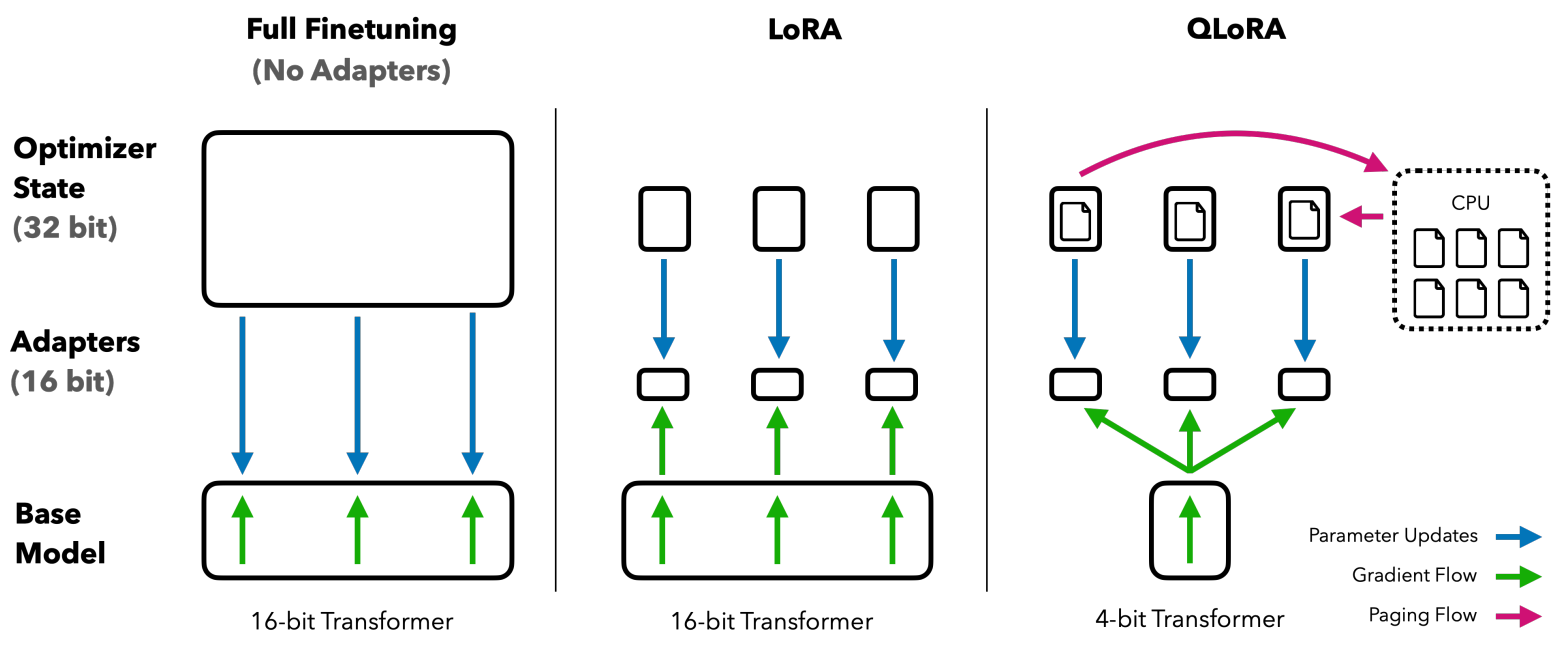
\includegraphics[width=5in]{qlora.png}
	\centering
	\caption{Difference in finetuning methods. QLoRA supplements LoRA by applying quantization to the transformer model. \cite{dettmers2023qlora}}
	\label{fig:qlora}
\end{figure*}

This year, Liu et al. (2024) proposed DoRA (Weight-Decomposed Low-Rank Adaptation), which introduces a weight decomposition analysis to investigate the inherent differences between FFT and LoRA \cite{liu2024dora}. DoRA decomposes pretrained weights into magnitude and directional components, using LoRA specifically for directional updates. This decomposition approach enhances both learning capacity and training stability compared to standard LoRA, while maintaining the advantage of no additional inference overhead. Their analysis revealed that DoRA exhibits learning patterns more similar to FFT than LoRA does, leading to improved performance across various tasks and model architectures.

\section{Methodology}

We ran a survey experiment on LoRA and QLoRA as efficient parameter tuning methods against a semantic evaluation problem. For our problem, the data was formatted similarly to the E2E NLG dataset \cite{novikova2017e2e}. We are given a set of labels and a string of text, and we format as such:
\begin{verbatim}
<text> <tech:> <labels,comma delimited>
\end{verbatim}

During training, this is tokenized and sent as both the input and labels for the model. Then, during inference, the labels are removed and the model performs next token generation on the text. Initial experiments were run on Llama 2-7B. The intention of choosing this model was motivated by the goal of demonstrating accessibility through PEFT methods. In general, the overall performance of the model is an interesting metric of how well PEFT is working, but the fact that an otherwise intractable problem like finetuning a 7 billion parameter model on consumer hardware could become possible through PEFT was the most desirable outcome. However, to gain a frame of reference for how the performance changed across PEFT methods and FFT, experiments were also run on Llama 3.2-1B.


\section{Experimental Settings}

Pre-trained models were acquired through HuggingFace by means of the \textbf{transformers} library, which integrates nicely with pytorch. Llama-3.2-1B and Llama-2-7B were selected as models to cover the range of appropriate sizes. Though 13B parameters is technically feasible with enough quantization, we would be stretching our resources such that it wouldn't properly compare to other results - for this reason, we focused solely on the 1B and 7B sizes.

For purposes of both adhering to the original literature and for optimality, certain choices were made for selecting the hyperparameters for the fine-tuning methods. LoRA adapters were applied to $Q$ and $V$ modules with a rank of 8 and alpha of 32. This was found successful in \cite{hu2021lora}, as it offers a balanced tradeoff of expressibility and efficiency. Additionally, from the suggestions of the success found in DoRA, we apply a LoRA dropout rate of 0.05\cite{liu2024dora}.

In our QLoRA model, we apply quantization using NF4, a 4-bit normal float representation that is shown to outperform other data representations of the same memory size. For computation of the gradient, weights are dequantized to bfloat16. Dequantization is, as mentioned in \cite{dettmers2023qlora}, often necessary for maintaining stability in the gradient during training. Also, we believe it's important to use an identical LoRA configuration for our QLoRA model in order to make a close comparison to the model without quantization.

\begin{figure}[h]
	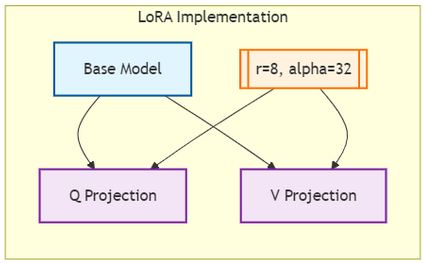
\includegraphics[width=\columnwidth]{lora_implementation.png}
	\centering
	\caption{Illustration of our application of LoRA adapters.}
	\label{fig:lora_impl}
\end{figure}

\begin{figure*}[h]
	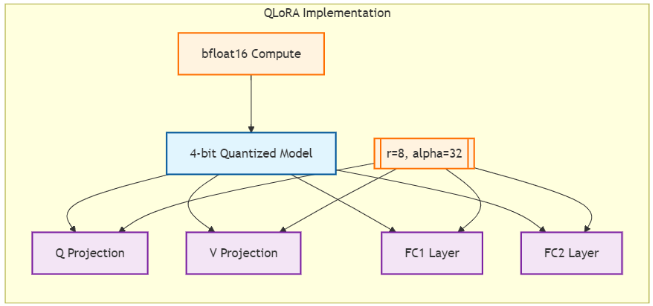
\includegraphics[width=5in]{qlora_implementation.png}
	\centering
	\caption{Illustration of our usage of QLoRA.}
	\label{fig:qlora_impl}
\end{figure*}

\section{Results}

\begin{table*}[h]
	\centering
	\caption{Comparison of LoRA and QLoRA on Llama 2 (7B) Model.}
	\label{tab:lora_qlora_comparison}
	\begin{tabular}{|l|c|c|c|}
		\hline
		\textbf{Llama 2 7B} & \textbf{Speed} & \textbf{Memory} & \textbf{Accuracy (F1)} \\ \hline
		FFT   & N/A      & N/A        & N/A        \\ \hline
		LoRA  & 62s/it   & 23.5 GB    & 0.441      \\ \hline
		QLoRA & 30s/it   & 14.6 GB    & 0.435      \\ \hline
	\end{tabular}
\end{table*}

The primary focus of this experiment is to show that model fine-tuning can be performed for tasks on consumer hardware, bypassing the need to rely on commercially-sourced cloud computing. In particular, we aimed to show performance increases for individual models on the tasks that were fine-tuned. Accordingly, our comparisons will be contrasted with the literature results for improved performance in both fine-tuning speed and memory performance. 
As explained in the previous sections, our computation was performed on an NVIDIA 3080TI with 12GB VRAM. The machine is set up to allow for a total of 44GB, by sharing 32GB of RAM with the GPU during computation. Therefore, we were limited to models requiring less than 44GB during training. The immediate result of this is that the fine-tuning of Llama 2 - 7B could not be performed without drastic improvements in the memory usage. This is in line with the core thesis of the research - in other words, we were not able to fine-tune a powerful model for a specific task without the implementation of LoRA or QLoRA, but with LoRA, it was possible to fine-tune these models in a reasonable amount of time. 

Table~\ref{tab:lora_qlora_comparison} shows the results of our initial finetuning task for Llama 2 7B. As is indicated by the FFT row, we were unable to fit the model into the 44GB system - assuming a 2x increase in memory requirements from the LoRA model, we would’ve needed about 47GB in order to fine-tune the 7B model. However, with a basic LoRA implementation, this memory requirement was effectively halved, resulting in a total memory usage of 23.5GB. From LoRA to QLoRA, we find an an additional decrease of ~37\% in memory usage, enabling the model to be fine-tuned on a GPU with only 16GB of VRAM. This shows a remarkable increase in accessibility from the original 44GB+ requirements of the base model.

We are unable to compare the speed (s/it), as the FFT model was unable to be implemented on our system. We expect that the speed would be higher for the FFT model without LoRA, as is evidenced by the results for the 1B model. There is an expected increase in speed between the LoRA and QLoRA implementation, matching the results from the literature [3]. It is difficult to estimate the difference in accuracy between the 7B FFT and LoRA results; however, we expect that the FFT model would have a higher F1 score than the LoRA model, based similarly on the results in the literature [1, 3].


Table~\ref*{tab:lora_qlora_3_2} shows the results for our experimentation with Llama 3.2 1B. Similar to the results for the 7B Llama 2 model, we find a roughly 2x decrease in the memory requirements for the LoRA implementation from the FFT implementation. The QLoRA implementation sees a further decrease in the memory requirements for fine-tuning, bringing the total requirement down to slightly over 4GB, enabling training on a standard, non-enthusiast consumer GPU. As expected, the LoRA implementation does result in a decrease in the speed of the training compared to the FFT implementation, while the QLoRA implementation improves marginally the training speed. Interestingly, we see a significantly lower accuracy for the full non-LoRA model, while LoRA and QLoRA see much higher F1 score. We do not see a corresponding improvement of this form in the literature, so we feel that this may be a quirk of the Llama 3.2 1B model.

\begin{table*}[h]
	\centering
	\caption{Comparison of LoRA and QLoRA on Llama 3.2 (1B) Model.}
	\label{tab:lora_qlora_3_2}
	\begin{tabular}{|l|c|c|c|}
		\hline
		\textbf{Llama 3.2 1B} & \textbf{Speed} & \textbf{Memory} & \textbf{Accuracy (F1)} \\ \hline
		FFT   & 1.26 it/s & 11.8 GB & 0.047 \\ \hline
		LoRA  & 7 it/s    & 5.63 GB & 0.076 \\ \hline
		QLoRA & 5.36 it/s & 4.09 GB & 0.073 \\ \hline
	\end{tabular}
\end{table*}


Figure~\ref{fig:leaderboard} shows the leaderboard results for SemEval 2021, Task 6, Subtask 1, which is the target task for our finetuning. We find that our fine tuning with LoRA and QLoRA of Llama 2 - 7B results in significantly higher performance than the baseline, performing well against the other leaderboard results. In contrast, we find that the FFT implementation of Llama 3.2 - 1B scores worse than the baseline, while the LoRA and QLoRA models perform slightly better than the baseline performance on the task. We are surprised at the poor performance of the FFT model, but are not surprised that the relatively small 1B model results in only marginally better than baseline performance.

\begin{figure}[h]
	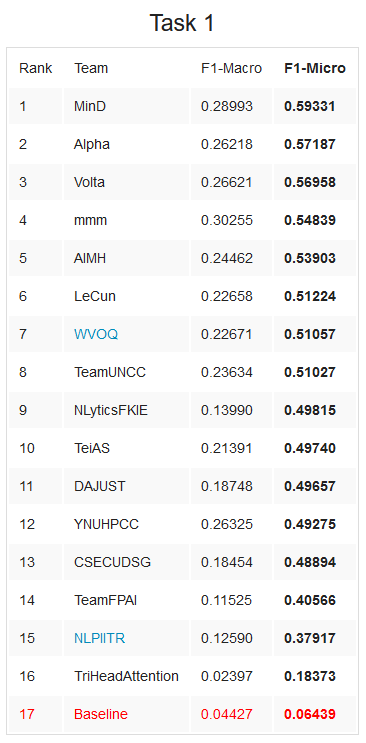
\includegraphics[width=2in]{semeval_leaderboard.png}
	\centering
	\caption{Leaderboard results from various team implementations for SemEval 2021 - Task 6, Subtask 1. The baseline performance is 0.06439. All of our implementations beat the baseline performance, besides the Llama 3.2 - 1B FFT implementation, which resulted in poor performance.}
	\label{fig:leaderboard}
\end{figure}

\section{Discussion and Notes}

The results of our fine-tuning on Llama 2 7B, which we were notably unable to perform on the FFT model without LoRA and QLoRA, shows that fine-tuning of LLMs can be implemented on consumer hardware. The inability to perform FFT without LoRA is a significant example of the typical limitation on consumer hardware, as the base model requires over 44GB for a simple fine-tuning run. We’re pleased to see that the LoRA and QLoRA implementations were not only successful, but beat the baseline on the SemEval Task 6, Subtask 1 leaderboard by a significant margin, with only a small run-time for the fine-tuning. While we were unable to compare the performance with the FFT model, this limitation is exemplary of the fundamental limitations on consumer fine-tuning of model
s. 
Interestingly, the comparison of our results for Llama 3.2 1B showed a reduction in performance for the FFT case compared to LoRA and QLoRA. This does not match the expectations from the literature, as it is expected that the FFT model will typically exhibit better performance than the LoRA and QLoRA model. We expect that this discrepancy arose from quirks with the Llama 3.2 1B model, and should not be assumed to be characteristic of all LoRA and QLoRA implementations. In contrast the training time and memory requirements match the results from the literature: training time increases from FFT to LoRA, but decreases from LoRA to QLoRA, whereas memory requirements consistently drop from FFT, to LoRA, to QLoRA. 

One thing that should be noted is the ease of implementation for QLoRA as an addition to LoRA. LoRA is already a fairly simple method to implement into machine learning pipelines. The inclusion of quantization into LoRA only required a single class to be called in the model definition, as explained in Appendix~\ref{sec:appendix}.

It is noteworthy how straightforward this implementation is. With a parameter configuration from the BitsAndBytes sub-package of transformers, the memory requirements for model finetuning are reduced by over 60\%. This verifies the fundamental premise of our research project, which is that QLoRA can be used as a simple, straightforward and capable solution to LLM fine-tuning on consumer hardware.

\section{Conclusion}

The memory requirements for the fine-tuning of LLMs is a significant barrier to entry for consumers, independent researchers, and enthusiasts, as it tends to require available memory well beyond the capabilities of standard consumer GPUs. While cloud computing solutions exist, these tend to be expensive to use for any extended period of time, and are often limited by low supply for consumers. As an alternative, LoRA and QLoRA have been proposed as solutions for consumers to fine-tune LLMs on local hardware. In order to test the accessibility of this method for consumers, we have successfully implemented LoRA and QLoRA on Llama 2 7B and Llama 3.2 1B, with the fine-tuning task of SemEval 2021, Task 6, Subtask 1 as a target metric. This successful implementation, which improved upon the leaderboard results from the 2021 task, and beat the baseline performance for most implementations, shows that LoRA and QLoRA are possible solutions for consumers attempting fine-tune models without excessive use of cloud computing services.

\section{Future Work}
Next steps of investigating the effectiveness and feasibility of PEFT methods can go in a few directions. The first would be to implement and make comparisons with other LoRA analogs, such as QLoRA-A. In conjunction with this, it also seems prudent to perform evaluation of different model architectures, and of various sizes suitable for commercial PC setups, such as state space models (SSMs) like Mamba. There are promising developments in making such models more efficient with fewer resources, with motivations mainly for the goal of improving cloud-serving\cite{quamba}; however, it should also serve to make said models more accessible for fine-tuning.

Regarding our application of PEFT techniques to address the SemEval task, while we achieved scores adequate to place on the leaderboard, we could explore different strategies apart from focusing on fine-tuning of the model. We left room for future investigations of using different prompting strategies, which includes but is not limited to employing Chain-of-Thought, Tree-of-Thought, and Retrieval-Augmented-Generation. The latter could especially have high impact, as the task involves memes, which evolve quite rapidly in both form and content - in order to effectively decide what is and is not propaganda, it seems intuitive that having any recent context, whether it be news or definitions of modern slang, could be vital.

Further valuable work would be tackling the multi-modal task, which considers the image and text in tandem. Li demonstrates practical results of using LoRA for multi-modal tasks, which can be investigated for this task \cite{li2024instruction}.

\section{Contributions}

Review of literature and writing of the report was done collectively, while some tasks were done individually, albeit with some collaboration and discussion.

Caleb was responsible for the writing of various scripts, and for running and debugging model training and evaluation.

Morgan wrote evaluation scripts for the pipeline, and was also responsible for formulating the fine-tuning script that utilizes the SemEval dataset.

Nick pieced the pre-trained models together and was responsible for writing the scripts to configure them for various fine-tuning methods, primarily LoRA adapters and quantization.

\bibliographystyle{acl_natbib}
\bibliography{references}

\appendix

\section{Quantization Implementation}
\label{sec:appendix}
To apply quantization to a model, the BitsAndBytes library is used to construct the desired configuration upon loading a model from HuggingFace.

\begin{lstlisting}[language=Python, caption={NF4 Quantization Configuration}]
nf4_config = BitsAndBytesConfig(
	load_in_4bit=True,
	bnb_4bit_quant_type="nf4",
	bnb_4bit_use_double_quant=True,
	bnb_4bit_compute_dtype=torch.bfloat16
)
\end{lstlisting}

When loading a model from HuggingFace, we apply the configuration as so:

\begin{lstlisting}[language=Python, caption={Loading a Quantized Model}]
model = AutoModelForCausalLM.from_pretrained(
	hf_model_name,
	quantization_config=nf4_config,
	device_map="auto"
)
\end{lstlisting}


\end{document}
